\documentclass[10pt]{report}

\usepackage[utf8]{inputenc}
\usepackage{amsmath}
\usepackage[acronym,toc]{glossaries}
\usepackage{graphicx}
\usepackage{hyperref}
\usepackage{booktabs} %for the use of Pandas tables outputed as latex

\title{Predictive Models on Tesla Stock}
\author{Samuel Sekarski \\ Supervisor: Dr. Gholam}
\date{June 2021}

\makeglossaries
\newacronym{ts}{TS}{Time Series}
\newacronym{ml}{ML}{Machine Learning}
\newacronym{tsla}{TSLA}{Tesla Stock}
\newacronym{gt}{GT}{Google Trends}
\newacronym{knn}{KNN}{k-nearest neighbors}
\newacronym{ann}{ANN}{Artificial Neural Network}
\newacronym{lm}{LM}{Linear Model}
\newacronym{dt}{DT}{Decision Tree}
\newacronym{rf}{RF}{Random Forest}
\newacronym{et}{ET}{Extremely Randomized Trees}
\newacronym{mse}{MSE}{Mean Square Error}
\newacronym{ar}{AR}{Autoregressive}
\newacronym{ma}{MA}{Moving Average}
\newacronym{arma}{ARMA}{Autoregressive Moving Average}
\newacronym{arch}{ARCH}{Autoregressive Conditional Heteroskedasticity}
\newacronym{garch}{GARCH}{Generalized Autoregressive Conditional Heteroskedasticity}
\newacronym{acf}{ACF}{Auto-correlation function}
\newacronym{pacf}{PACF}{Partial auto-correlation function}
\newacronym{ols}{OLS}{Ordinary Least Squares}


\newglossaryentry{API}
{
	name=API,
	description={tools available for interfacing with a library}
}
\newglossaryentry{R2}
{
	name=$R^2$,
	description={Coefficient of determination}
}
\newglossaryentry{snp}
{
	name=S\&P500,
	description={S\&P500 index, composed of 500 important US stocks}
}

\begin{document} 
\maketitle

\tableofcontents
\listoffigures

\chapter{Introduction}
%Questions:
%ML vs TS ?
%What support data could improve accuracy ?
%In summary on ISA i wrote "how did covid impact stock price", buuuut didn't really look at that (yet ?)
%Supervisor said to make it a bit more about financial time series in general
In 2020, despite the global pandemic, the electric vehicle maker Tesla saw it's stock price go up 700$\%$, which is more than Amazon's or Netflix's went up, both of whom profited during the pandemic. Tesla was also added to the S$\&$P500 index in November and underwent a stock split shortly before that, because of increased demands. In fact for years, Tesla stock has been on the minds of more and more potential investors, wondering if they should buy-in or not.

In this thesis, we will look to try to find models that could accurately fit Tesla's stock price evolution, which people could use to help make decisions. We will not, however, develop any kind of trading strategy, nor suggest to the reader any financial actions.

To frame our research our main question will be: How well can existing models fit Tesla stock price ?
We shall use data spanning 2019 and 2020.

The classical approach to financial data is through \acrfull{ts} analysis, and as such we shall consider various models developed for time series. The more novel approach is to use \acrfull{ml} algorithms to attempt to train a model to fit the financial data. We shall explore some of these methods as well, and then compare both the Machine Learning and Time Series approaches, and see which yields the better fits. This shall be our second area of focus.

In continuation of the first question, we shall ask ourselves how public sentiment about Tesla affects it's stock. In the past, investing was reserved only to big institutions and select individuals, but with the rise of internet, this practice has been expanded and now anyone (so called "retail investors") can invest. And as seen in the Gamestop short squeeze of January 2021, when a group of individuals have a similar sentiment, they can influence the markets immensely. We shall use Google Trends to see if adding a public sentiment factor into account benefits the modelling.

Another subquestion we shall consider, is whether posts on social media can influence a stock.
Tesla CEO Elon Musk is known for his tweeting habits that can shake markets, as for example with his tweets about cryptocurrency in early 2021. Another example, closer to the subject, is when Musk tweeted in May 2020 that the stock price was "too high" and the stock then fell 10$\%$. The US Securities and Exchange Commission (SEC) definitely thinks Musk's tweet have influence, as the SEC filed a lawsuit against the billionaire in September 2018 regarding one of his tweets \footnote{\url{https://www.sec.gov/news/press-release/2018-226}}. We shall use data collected from Twitters API to see if his tweets truly have an influence and if using this data we can improve upon our models.


We shall also, in a lesser measure, compare how implementations of these methods in the two main programming languages for data analysis, that is Python and R, compare to each other. Are there significant outcome differences using one or the other ? What kind of support (frameworks, libraries, packages, etc.) exist for this kind of modelling in each ?

And finally, since the beginning of 2021, the stock price has tapered off, and fallen. We shall lastly ask ourselves if our best models developed on the 2019 and 2020 time frame will predict this.

\chapter{Tools}
\label{chap:tools}
%Python,R - Quels packages, libraries, etc.
\Gls{python} will be our main tool for analysis, but we will also consider using \Gls{r}, and compare, where appropriate, the results using \Gls{python} versus using \Gls{r}, to see if there are any differences in implementation that influence the outcome of our analysis.

\section{\Gls{python}}
\Gls{python} is a multi-purpose high level programming language, which is gaining a lot of traction in the \acrlong{ml} community, for its simple syntax and library support.
The main package we will be using for \acrlong{ml} is 'sklearn' \footnote{\url{https://scikit-learn.org} (June 24, 2021)}.
The main pacakge we will be using for \acrlong{ts} is 'statsmodels' \footnote{\url{https://www.statsmodels.org} (June 24, 2021)}.
For \acrshort{garch} we will use the 'arch' package \footnote{\url{https://arch.readthedocs.io} (June 24, 2021)}.
For data manipulation we will be using 'pandas' \footnote{\url{https://pandas.pydata.org} (June 24, 2021)} and 'numpy' \footnote{\url{https://numpy.org/} (June 24, 2021)}.

\section{\Gls{r}}
\Gls{r} is a programming language designed specifically for statistical computing and graphics and has been the go-to programming language for data scientist in the past. It has a lot of library support as well.


The main package used is 'tidyverse' \footnote{\url{https://www.tidyverse.org} (June 24, 2021)}. This is actually a collection of packages, that all share the same underlying structure, and that are data science orientated.


For \acrshort{garch} modeling we will be using the 'fGarch' package \footnote{\url{https://cran.r-project.org/web/packages/fGarch/index.html} (June 24, 2021)}.

\chapter{Data}
%présentation des datas, à quoi ça ressemble, preprocessing, data auxiliaire
Realizing that we need to be careful with time zones, as for example, TSLA is traded on the NASDAQ stock exchange, which is in New York, whereas Elon Musk tweets from California and I am in Switzerland while analysing the data and the reader might be anywhere in the world, we shall convert all times to UTC.
\section{Main data: Tesla Stock Price}
The \acrshort{tsla} price data was retrieved using the python package "yfiance" which makes calls to the Yahoo Finance \Gls{API}. We were able to download 730 days worth of hourly data, spanning the last 730 days from download date. The Yahoo Finance \Gls{API} is not being maintained, so this may not be possible in the future. The data was retrieved on February 10th 2021 and spanned from February 11th 2019 at 00:00 till February 10th 2021 at 00:00.
The raw data contained the following variables: "Open", "High", "Low", "Close", "Volume", "Dividends" and "Stock Splits".
For the purposes of this thesis, we only kept "Open" which was an arbitrary choice.

\begin{figure}[h]
	\centering
	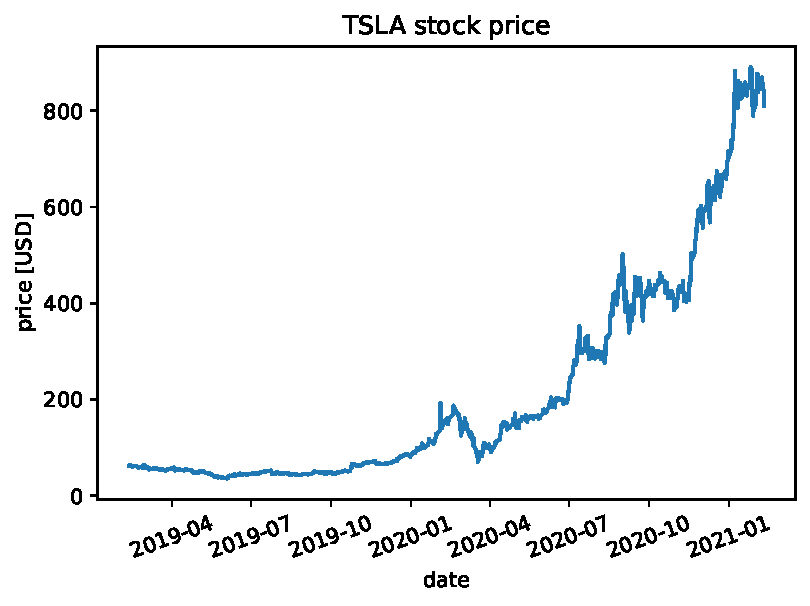
\includegraphics[width=\textwidth]{img/img_tsla.pdf}
	\caption{TSLA hourly opening stock price}
	\label{fig:tsla_open}
\end{figure}



\section{Auxiliary data}
\subsection{Google Trends}
\acrfull{gt} is a tool that lets researchers explore how the Google search engine as been used. We shall use the search term "tesla" in the explanation and graphics, as the other search terms ('tsla', 'tesla stock' and 'musk') were similarly preprocessed.

\begin{figure}[h]
	\centering
	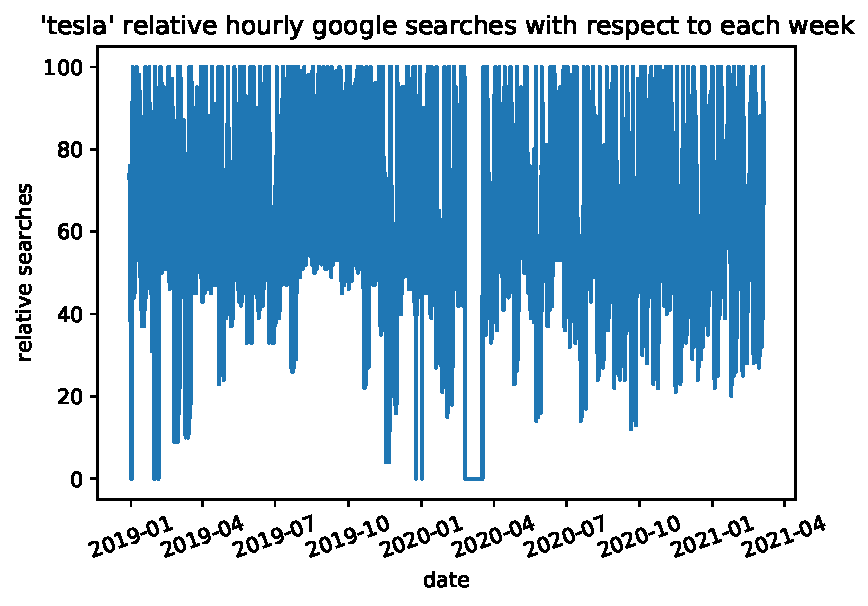
\includegraphics[width=\textwidth]{img/img_GT_tesla_raw.pdf}
	\caption{Hourly google searches of the term "tesla" relatively to each week, in percentage of the weekly maximum}
	\label{fig:GT_tesla_raw}
\end{figure}


The \acrlong{gt} data was retrieved using the python package "pytrends" which makes calls to the \acrlong{gt} \Gls{API}. Each \Gls{API} call will return the percentage of the number of searches per time unit in an interval, relative to the peak searches of the interval. That is to say that at the time step where there were the most searches, the returned value will be 100, and for all other time steps, the return value will range from 0 to 100, rounded to the nearest digit.
We are interested in hourly data, but for hourly granularity, we can only retrieve one week at a time. Retrieving a longer interval results in a higher granularity. The solution we used was to do multiple calls to the \Gls{API} to get the hourly data relative to each week, and then also retrieve the weekly-granular data for the entire timeframe, and compose the hourly with the weekly, to get hourly percentage relative to the whole time interval.

The data was retrieved on March 17th 2021 and spanned from December 31st 2018 at 06:00 to March 17th 2021 at 15:00.
After visual and numerical inspection of the data (fig \ref{fig:GT_tesla_raw}, it appeared that there was a gap in the data between February 24th 2020 12:00 and March 17th 2020 15:00. I can only hypothesis that there was some Covid-19 induced problem at Google that is responsible for this, as that's the time frame where the Pandemic started to really pick up globally, as the same gap is present in all searches that I looked up with their \Gls{API}. 
We truncated this missing data, with the daily \acrshort{gt} value, which were available. We did a simple step truncation, before composing the hourly-weekly data with the weekly-interval data. As shown in Fig \ref{fig:GT_tesla_probarea}

\begin{figure}[h]
	\centering
	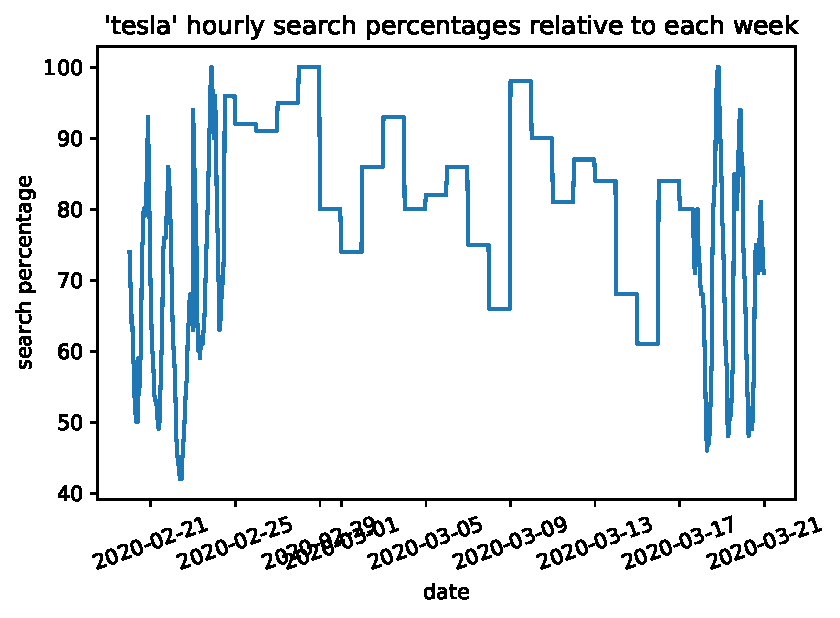
\includegraphics[width=\textwidth]{img/img_GT_tesla_probarea.pdf}
	\caption{Google searches for "tesla" between February 20th and March 20th 2020, where the missing hourly data as truncated with daily data}
	\label{fig:GT_tesla_probarea}
\end{figure}

We observe in this figure also, that there seems to be some daily periodicity in the searches, which is explained by the fact that we only looked at searches done in the United States, so during night time hours it makes sense that there would be less searches.
%Note to self: should I detrend the data ? Or should I look for exceedences over a threshold or some other maxima scheme ??


As the trading data is only between 10am and 5pm EST, we simply dropped data outside of that fork. This was a subjective choice, and it can be discussed whether it would not have been better to aggregate the dropped time and incorporate them in the observations somehow. Our reasoning was that if people searched for the terms before the market opening (say at 11pm the previous day), because they were interested in buying, they were likely to search for the term again right before the market opens, in order to make sure no new information came to light in the mean time to change their mind, and thus their interest would still be captured in the used data. Likewise, if someone was searching with the intent on selling, they too would search again prior to making the transaction, in order to double check.

\begin{figure}[h]
	\centering
	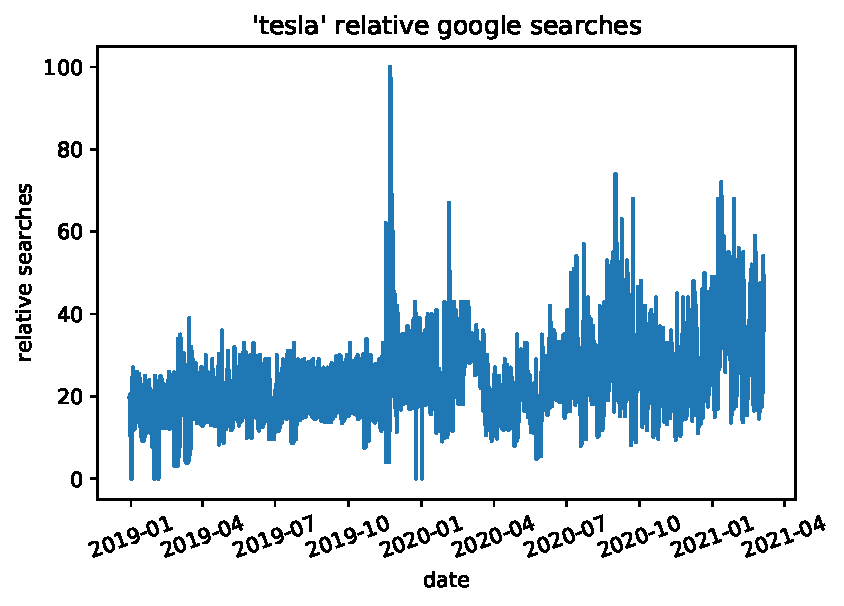
\includegraphics[width=\textwidth]{img/img_GT_tesla.pdf}
	\caption{"tesla" keyword relative google searches}
	\label{fig:GT_tesla}
\end{figure}

The final preprocessed data can be seen in figure \ref{fig:GT_tesla}

\subsection{Twitter data}
The popular social media platform Twitter has an \Gls{API} that lets researchers interact with and explore the Twitter Database. There are several tiers available that give different degrees of access to the database. The free tier did not give significant access to the tweet history, and as such we had to apply for an academic tier.

The API gives access to an impressive amount of data. We will be focusing on tweets by Elon Musk, and twitter metrics of "like count" and "retweet count", though others are available as well. These are the most used metrics when judging a tweets popularity.
Even if they both measure a tweets popularity, if they are not very correlated it could be worth keeping both of them, as a like only shows approval of the tweet, whereas a retweet shows approval, but also spreads the tweet to a larger audience. So it could be used as a metric of how much a tweet has spread.However, upon inspection (Fig  \ref{fig:likeretweets}) the retweet count and the like count seem pretty correlated, so we will focus only on the like count which will be both a measure of the approval of the tweet as well as a measure of how viral it is.

\begin{figure}[h]
	\centering
	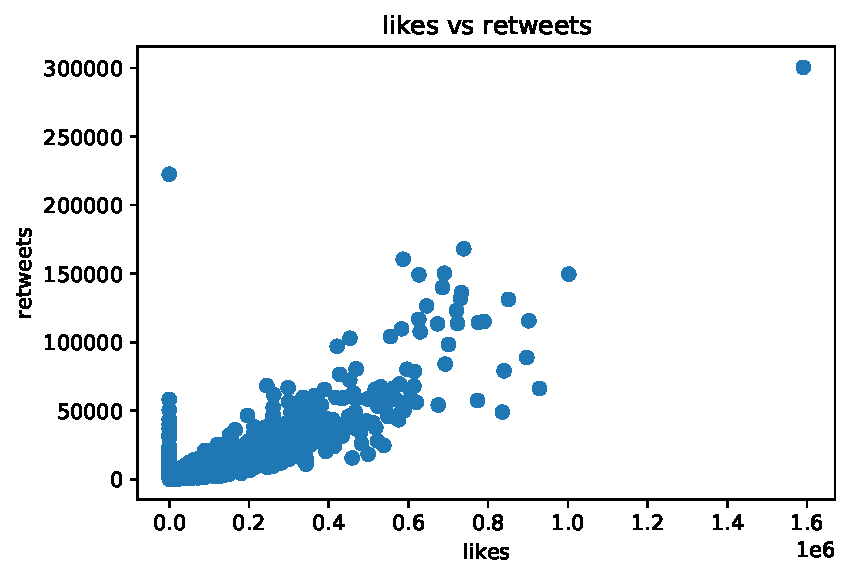
\includegraphics[width=\textwidth]{img/img_likeretweets.pdf}
	\caption{Elon Musk's tweets like count vs retweet count}
	\label{fig:likeretweets}
\end{figure}


Tweets have a precise timestamp and thus we have aggregated them to that for every hour H, the corresponding value is that of the sum of all tweets in the range ]H-1,H]. We then added the out of trading hours values to the first trading hour of each day. Again, it can be discussed whether it would have been better to aggregate this data differently, or drop it all together, like for the \acrlong{gt} data. Our reasoning is that if Elon Musk tweets something out of hours, that gets people in a good or bad frenzy about \acrshort{tsla}, then that frenzy would not die down before the market opened.

Elon Musk tweets a lot about things unrelated to Tesla and it's stock as well, so we will filter tweets with the term "Tesla". This may be too much filtering, as it could be imagined that other keep words could be worth adding to the filter, but it should be decent enough.

\begin{figure}[h]
	\centering
	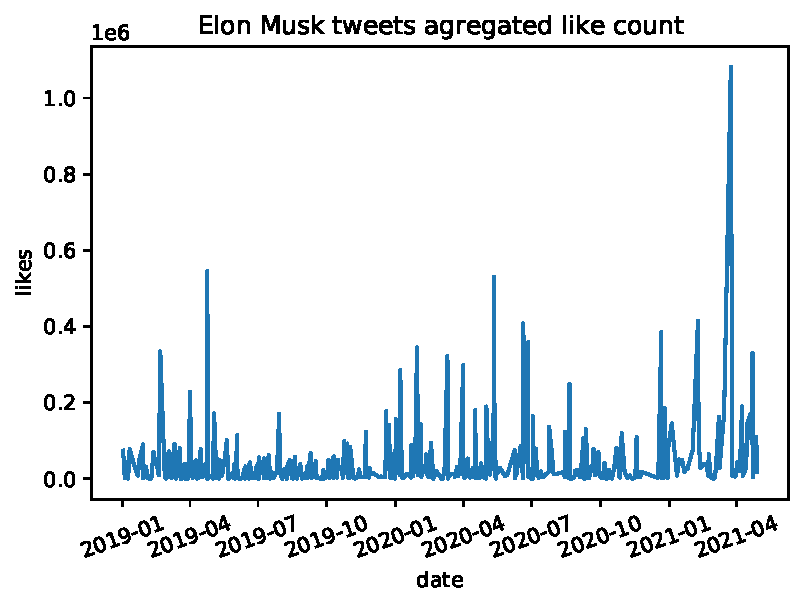
\includegraphics[width=\textwidth]{img/img_agglikes.pdf}
	\caption{Elon Musk's tweets like count, aggregated to fit the trading hours of NASDAQ}
	\label{fig:agglikes}
\end{figure}

The final aggregated like count per period can be seen on figure \ref{fig:agglikes}

\chapter{Experiment Design}
%need better name for this chapter. Can't remember what this is called when we're not actually doing experiments.
We shall separate all our data into 2 sets: the training set $(\mathcal{X}_{train},\mathcal{Y}_{train})$ and the test set $(\mathcal{X}_{test},\mathcal{Y}_{test})$
The split date was chosen to be January 4th 2021 at 10:00.
We will train our models on the training set, and then predict responses for observations in the test set. That is we will predict a set $\mathcal{Y}_{predict} = F(\mathcal{X}_{test})$ where $F()$ is the model's prediction function.

\section{Metrics}
%R^2
%MSE
%others ???

To compare the results and rank them, we shall use several metrics to asses goodness of fit and predictive power. The main two we shall consider are \acrfull{mse} and $R^2$.
\subsection{$MSE$}
Let $m$ be the size of the test set and let $\hat{Y}_i$ be the predicted value for the $i$-th observation in the test set.
The \acrlong{mse} is defined as $MSE(\mathcal{Y}_{predict}) = \frac{1}{m}\sum_{i=1}^m (Y_i - \hat{Y}_i)^2$
\subsection{$R^2$}
$R^2$ denotes the coefficient of determination.

The one used by our Python package, is defined as:

$R^2(\mathcal{Y}_{test},\mathcal{Y}_{predict}) = 1 - \frac{\sum_{i=1}^m(y_i - \hat{y}_i)^2}{\sum_{i=1}^m(y_i - \bar{y}_i)^2}$

Where $\bar{y} = \frac{1}{m} \sum_{i=1}^m y_i$. %(source (25.05.2021): https://scikit-learn.org/stable/modules/model_evaluation.html#r2-score)

The best score is 1.0, a constant model that always predicts the expected value of $y$ without taking into account the input, would be 0.0 and the score can be arbitrarily negative, as the top term can be arbitrarily large (i.e. our predictions can be arbitrarily bad. So for our methods to be better than just using the mean of the observations, we would like them to be larger than zero.

\section{set-up}
%ML univariate response: using one value of each feature for predict one value of response
%ML multivariate resposne: using one month of features are one point in the feature hyperplane to predict one week of responses as one point in the response hyperplane

\subsection{Univariate response}
In this set-up we consider the response variable to be univariate $Y=Y_t$.

We shall then train the models on the training set, and then predict one week ahead, and compare with the values of the test set.

\subsection{Multivariate response}
In this set-up we consider the response variable to be multivariate $Y=(Y_t, Y_{t+1}, ..., Y_{t+r})$
We shall consider the response to be one week ahead worth of data, or 35 steps. To predict this multivariate response, we shall augment the feature space dimensions, by not only considering $X_{j_t}$'s as predictors, but also $X_{j_{t-1}},X_{j_{t-2}},...,X_{j_{t-p}}$ as predictors. We shall consider one month of past data (or 140 time steps) as part of one observation.

In the first set-up, the forecast of observation $Y_{t+1}$ is generally good but the forecast of each observation after that gets more and more vague, faster and faster. To the point where after a number of time steps, the forecasts hold no more value and become effectively useless. The idea in the second setup, is to put a certain number of future observations into the response variable, so that when forecasting, the "first observation" that is forecast (so the one that is usually the best) now contains contains multiple steps ahead. Of course this comes at a price; using the same feature space, but with more response variables, will cause the fit and predictions to be worse. So we need to augment the feature space as well, by considering multiple steps behind as part of one observation point. This is actually what the Time Series methods actually already do. They use a combination of previous values to predict the next values.

We shall then train this on the training set, and predict one step ahead (which effectively will be one week ahead) and compare the values with those of the test set.


\chapter{Methods}
%LM,KNN,Tree,ANN,Garch - qu'est-ce que c'est et comment ça marche

\section{Time Series Methods}
\subsection{ARIMA}
\subsection{GARCH}

$$
Y_t = \sigma_t \epsilon_t
$$
$$
\sigma_t^2 = \alpha_0 + \sum_{j=1}^m \alpha_j Y_{t-j}^2 + \sum_{j=1}^r \beta_j \sigma_{t-j}^2
\quad, \epsilon_t \stackrel{iid}{\sim} \mathcal{N}(0,1)
$$

\acrshort{garch} models are generally the \acrlong{ts} models used for financial data

\section{Machine Learning Methods}
We'll go over the various methods we will be using, giving a brief description and overview of the pros and cons of each and when it is appropriate to use them.
We will suppose that there are $n$ observations and $m$ features.


\subsection{Linear Models}
The idea is to use a linear combination of features to determine the response. The linear constants are the parameters that need to be chosen to give the best approximation of the response space using the feature space. Geometrically this means fitting a hyperplane to the training set, by minimizing some function (loss function).
Formally:
$$
Y_j = \sum_{i=1}^m \beta_{i} X_{ji} \quad, j=1,\dots,n
$$

\subsubsection{Advantages}
\acrlong{lm} are some of the most common and simple models out there, but they have proven to be reliable and can be made quite complex with feature engineering. There plenty of theory and proofs about these methods. This all makes these methods and obvious first choice of methods to consider.
%insert "toute est linéaire" quote
\subsubsection{Problems}


\subsection{K Nearest Neighbours}
The intuition behind \acrshort{knn} methods is simple. The idea is that observations (points in the feature space) which are "close" will have responses that are also "close". Then a good approximation would be given by averaging the responses of the K observations "closest" to the new observation.
In this model, we need to chose the definition of "close" as well as chose the value of K.
Usually, the distance used to define close, is the euclidean distance and that is the one we used. As for K this parameter needs to be tuned. The larger it is the smoother the result is and the lower the more jagged it is. For optimal tuning the parameter should be as small as possible, without over-fitting.
\subsubsection{Advantages}
It's very intuitive and very simple to implement. 
It's non parametric ? <- no prior knowledge or guess about the prior distribution
\subsubsection{Problems}
It suffers from curse of dimensionality. When the dimension of the feature space gets large, the space becomes sparsely populated, and the K closest observations, might actually be very far from each other, and thus not reflect well the new observation.
As a workaround for this problem, there is a variant of \acrshort{knn} which instead of using the K closest observations, uses all the observations which fall in a certain radius of the new observation point. Thus the K parameter becomes R, the radius of the hyperball.
\subsection{Trees}
\subsection{Artificial Neural Networks}

\chapter{Results}
%comparaison, metriques. graphs

\section{Time Series Approach}
As the methodology to arrive to the final model is the same in R and Python, we will just layout the Python version in detail, and then state the final result using R.

\begin{figure}
	\centering
	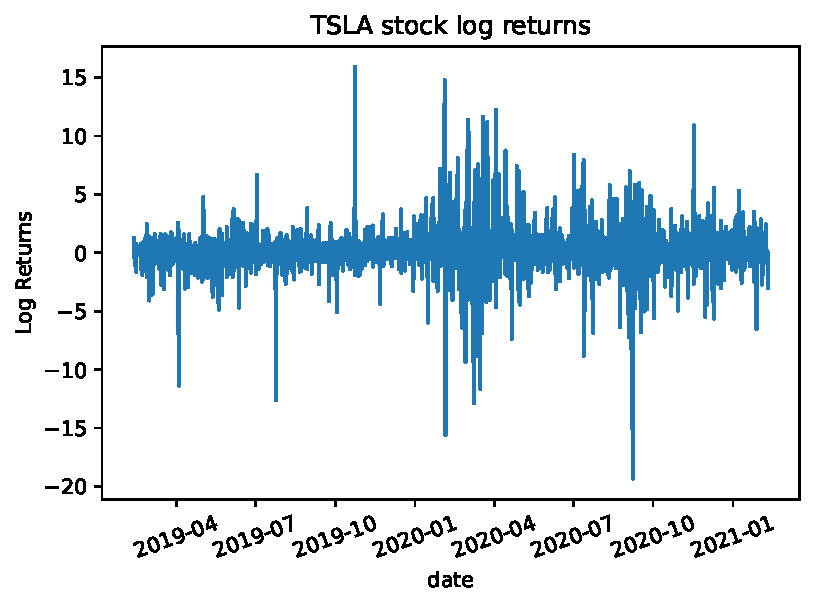
\includegraphics[width=\textwidth]{img/img_returns.pdf}
	\caption{Log returns of TSLA hourly opening stock price}
	\label{fig:tsla_returns}
\end{figure}

As financial data is not stationary and exhibits non-linear trends, and potentially heteroskedasticity, it is common practice to consider the log returns of the series. That is, to consider the series $X'_{t+1} = 100[ln(X_{t+1})-ln(X_t)]$. We see that in Fig \ref{fig:tsla_returns} the returns seem to be stationary. We check this by considering the \acrshort{acf} and \acrshort{pacf} graphs of the returns.

\begin{figure}
	\centering
	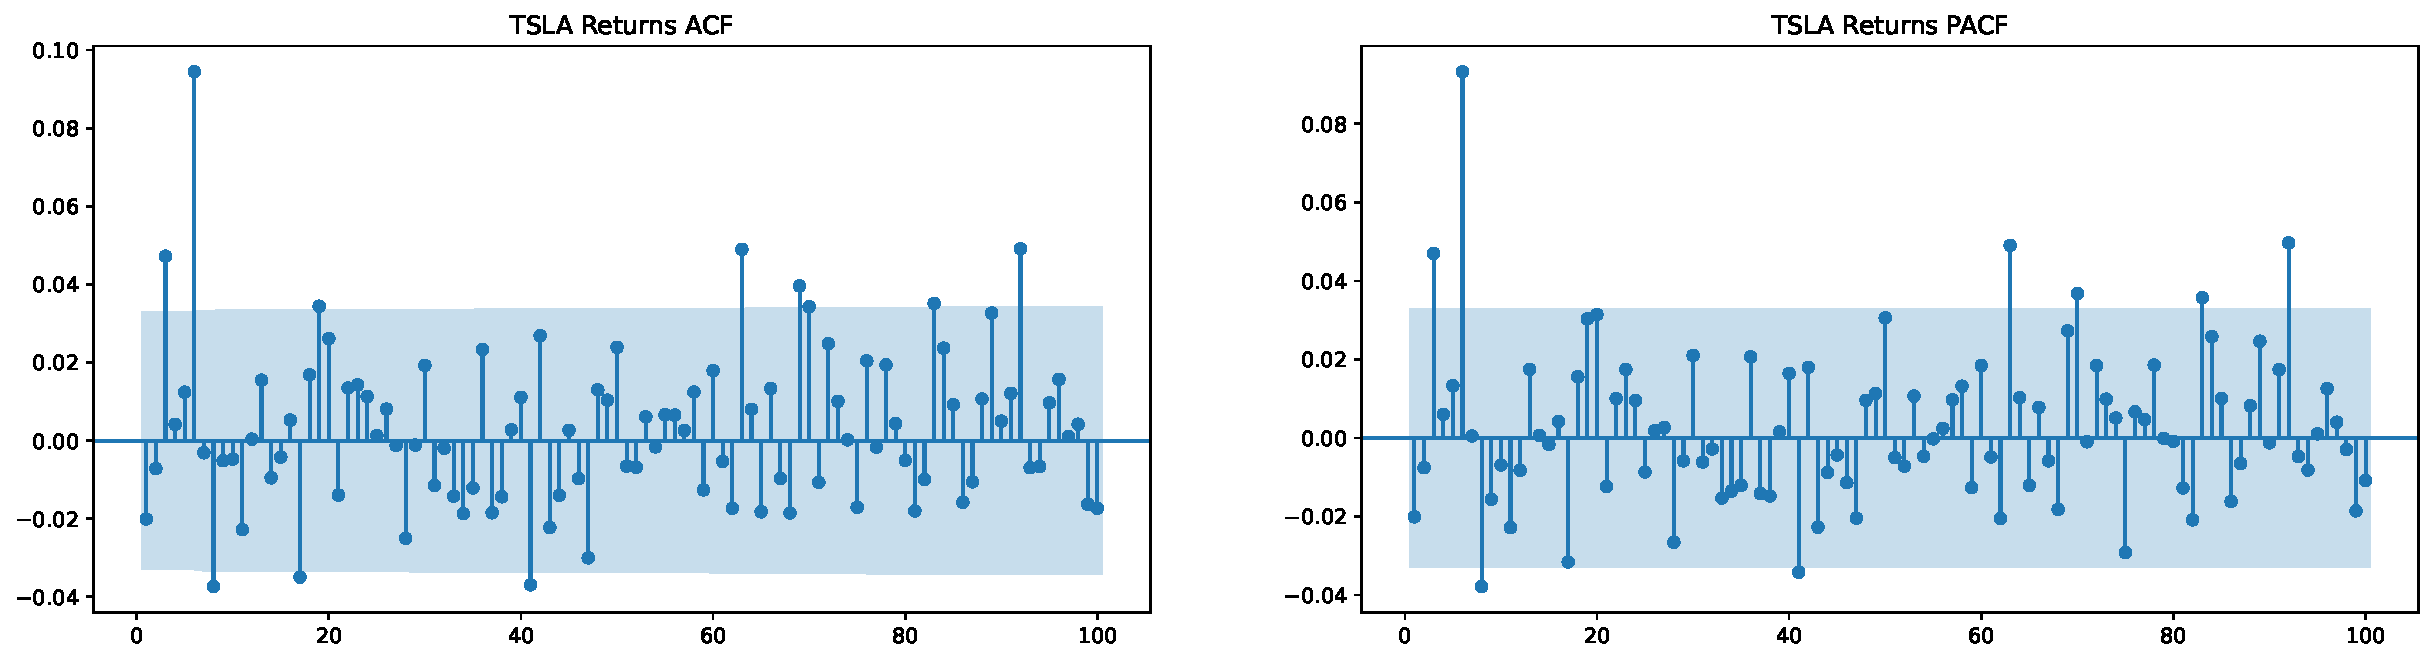
\includegraphics[width=\textwidth]{img/img_acf_tsla.pdf}
	\caption{\acrshort{acf} plot of log returns of TSLA stock price}
	\label{fig:acf_returns}
\end{figure}

Looking at Fig \ref{fig:acf_returns} there are a few lags that fall out of the 95\% significance interval. Oddly enough there would seem to be some significant autocorrelation at lag 6, which is surprising as if anything I would have expected there to be lag 7 autocorrelation, as there are 7 observations per day. It's not a very high autocorrelation nonetheless and fitting an \acrshort{arima} model with seasonality 6 just introduced more structure into the series instead of removing it, so we abandoned that path.

\begin{figure}
	\centering
	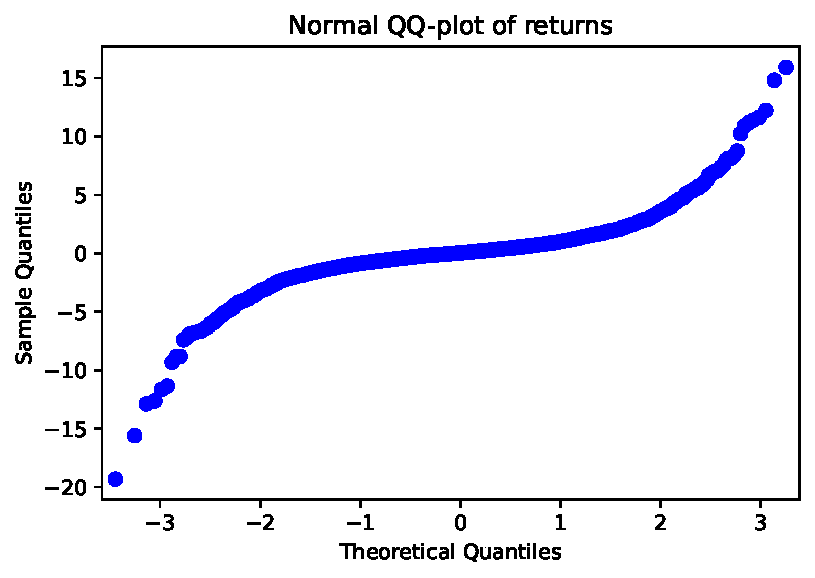
\includegraphics[width=\textwidth]{img/img_nqq_returns.pdf}
	\caption{Normal QQ plot of log returns of TSLA stock price}
	\label{fig:nqq_returns}
\end{figure}

We also checked the normal QQ-plot of the returns (Fig \ref{fig:nqq_returns}) and they are clearly not normally distributed. They have heavier tails, so we fitted a Student t distribution, manually tuned to a parameter $\nu = 2.6$ (Fig \ref{fig:tqq_returns}). This fits pretty well. At this point one could almost argue that the returns are just white noise with Student $t_{\nu}$ distribution.

\begin{figure}
	\centering
	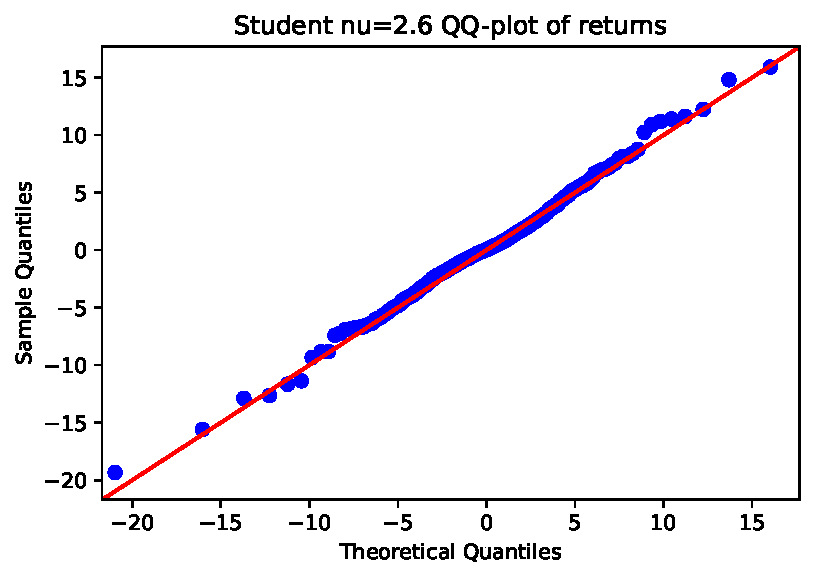
\includegraphics[width=\textwidth]{img/img_tqq_returns.pdf}
	\caption{Student QQ plot of log returns of TSLA stock price, with a parameter $\nu=2.6$}
	\label{fig:tqq_returns}
\end{figure}

However, when we look at the \acrshort{acf} and \acrshort{pacf} of the squared returns (Fig \ref{fig:acf_sreturns}, we notice distinct autocorrelation every lag multiple of 7. This suggest that there is significant structure in the volatility of the returns. This phenomena is called "volatility clustering" and happens a lot in financial \acrlong{ts}. The idea is that volatility breeds volatility; a period of volatility follows a period of volatility. 

\begin{figure}
	\centering
	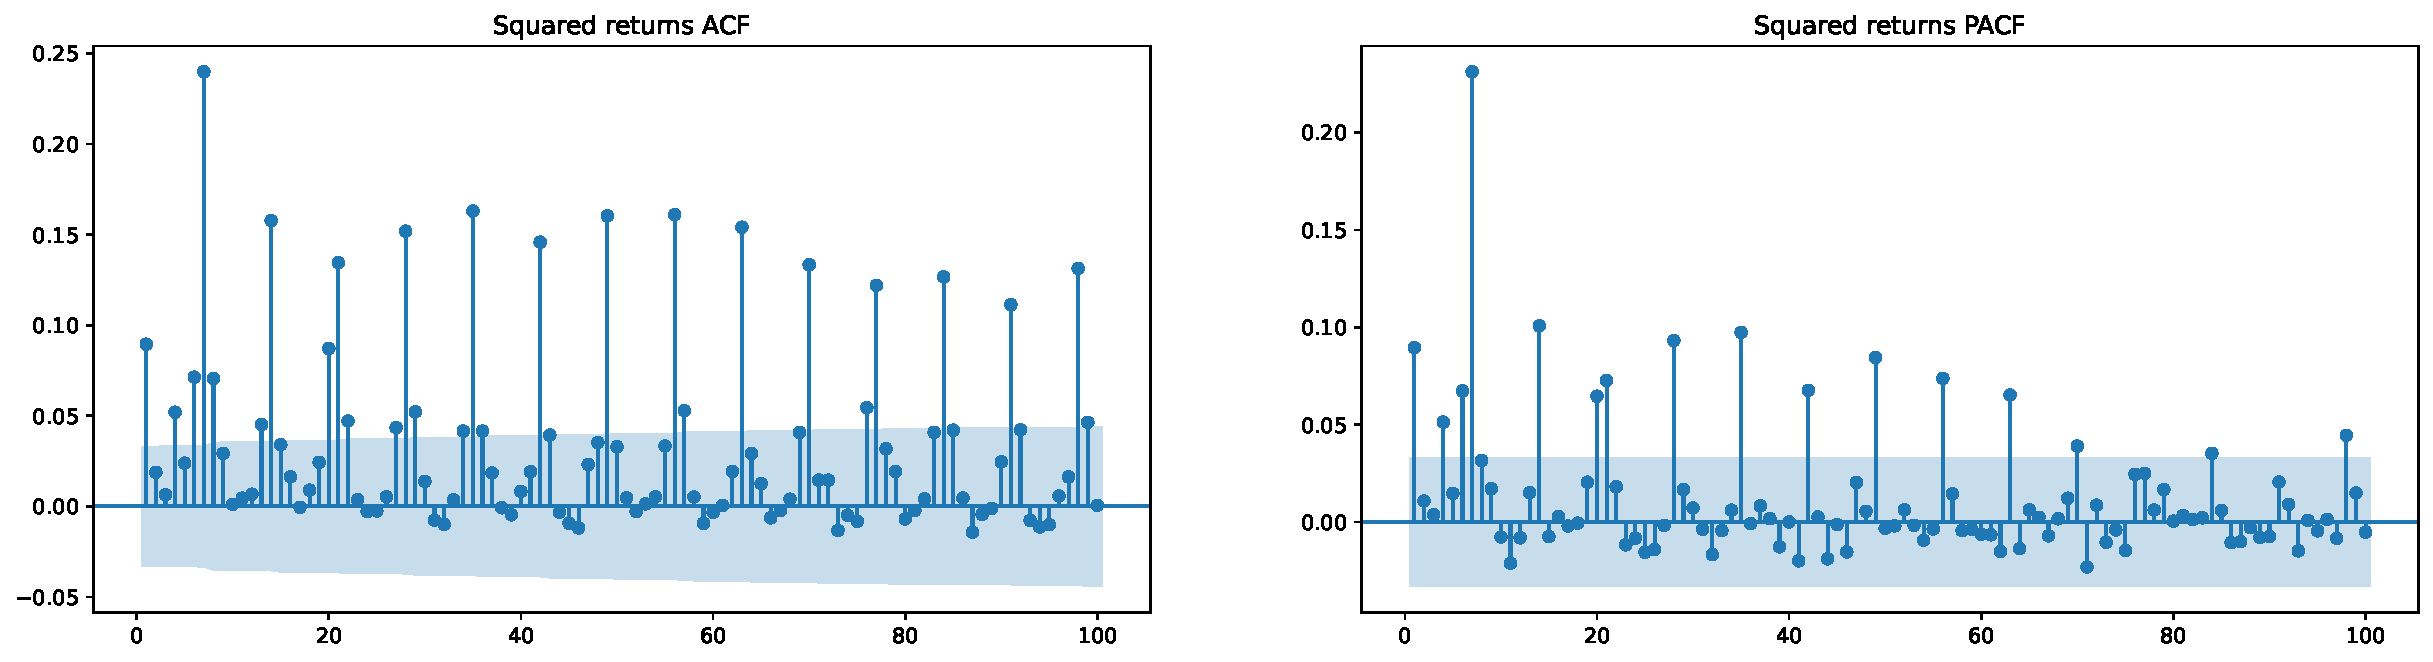
\includegraphics[width=\textwidth]{img/img_sreturns.pdf}
	\caption{\acrshort{acf} and \acrshort{pacf} of squared \acrshort{tsla} log returns}
	\label{fig:acf_sreturns}
\end{figure}

To model structure in the volatility of a series is where \acrshort{garch} model come into play. We first tried fitting a simple \acrshort{arch} model to the returns, but the results were not particularly better, so then we fit a \acrshort{garch}(1,1) with Student white noise model to the returns, and as you can see in figure \ref{fig:acf_sgarch} and figure \ref{fig:tqq_garch} the fit is very good.

\begin{figure}
	\centering
	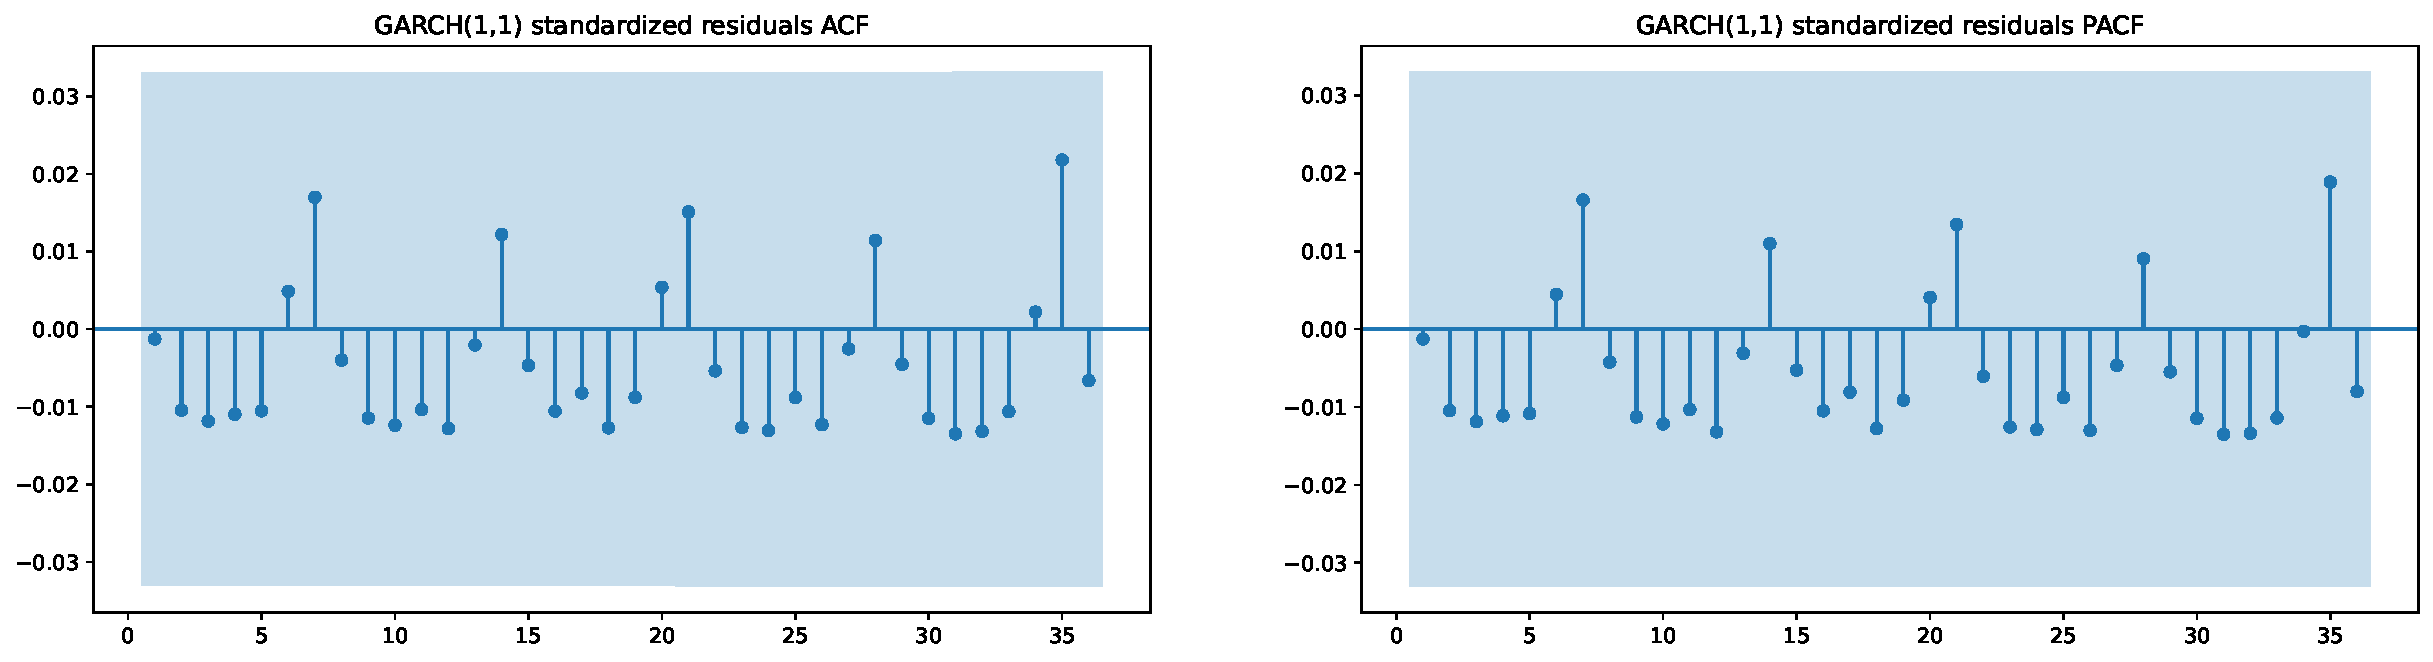
\includegraphics[width=\textwidth]{img/img_acf_garch.pdf}
	\caption{\acrshort{acf} and \acrshort{pacf} of squared standardized residuals from fitting a \acrshort{garch}(1,1) model with distribution $t_{\nu}$}
	\label{fig:acf_sgarch}
\end{figure}

\begin{figure}
	\centering
	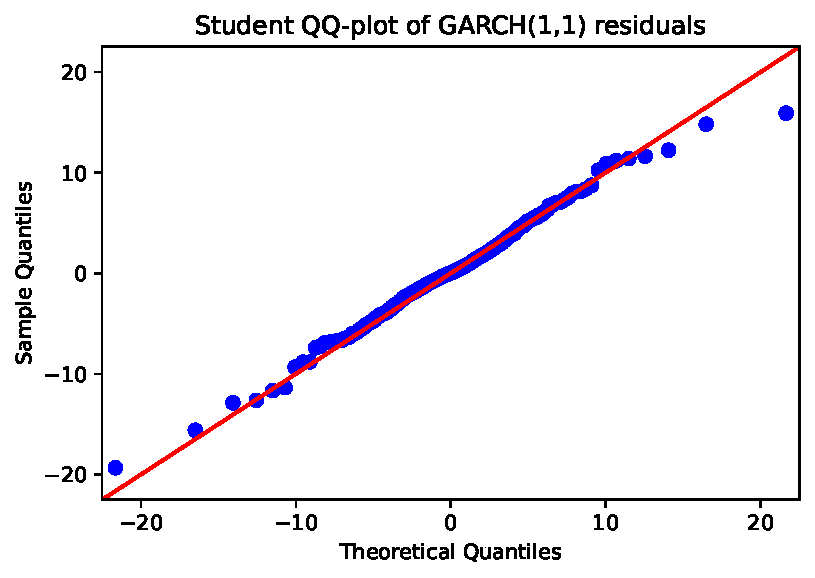
\includegraphics[width=\textwidth]{img/img_sqq_garch.pdf}
	\caption{Student QQ-plot of \acrshort{garch}(1,1) fitted to the \acrshort{tsla} returns}
	\label{fig:tqq_garch}
\end{figure}

The standardized residuals in figure \ref{fig:resid_garch} look very much like white noise now. Figure \ref{fig:resid_garch} also shows the conditional volatility extrapolated by the model. There are several things we see here. First, there is a large increase in volatility between January 2020 and May 2020, which I hypothesize is related to the uncertainty generated by the first wave of Covid-19. The later waves did not affect the volatility much, because by that time the initial panic had subsided, knowledge about the virus and how to fight it was more redly available. But that first wave caused havoc on the markets. The second thing we notice, is that there are spikes of very short duration but high value that happen every so often. They seem to be every 3-ish months and I would hypothesize that they more or less coincide with Tesla's quarterly earnings reports.
Indeed, according to Tesla's investors website ... \url{https://ir.tesla.com/}
The dates of the quarterly reports were:

\begin{tabular}{l}
Q4/18: Jan 30th 2019 \\
Q1/19: Apr 24th 2019 \\
Q2/19: Jul 24th 2019 \\% the website actually says Jun, which is a mistake. If clicked on it says Jul
Q3/19: Oct 23rd 2019 \\
Q4/19: Jan 29th 2020 \\
Q1/20: Apr 29th 2020 \\
Q2/20: Jul 22nd 2020 \\
Q3/20: Oct 21st 2020 \\
Q4/20: Jan 27th 2021
\end{tabular}


But this is not quite on point. First there is the case of Q1/20 which doesn't appear to have caused a spike in volatility, but this could just be that is was overshadowed by the Covid-19 first wave. Then there is Q4/20 that doesn't show up at the end of the graph. But as the other spikes are also a bit off from the quarterly report date, it's possible that the spike happens right after the end of the period we are considering, and that the spike are not fully explained by the quarterly report. Perhaps, when the spikes occur before the reports, it is because people are betting they will be good or bad, and there is excitement, maybe because a product launched that quarter or something. And when the spikes occur after the report, it could be because the reports were better or worse than expected, or maybe following a good report, Tesla or Elon Musk announce something big in the following days.
What's more, Tesla releases a press release basically 2 weeks prior to the earnings report. For Q4/18, this corresponds with the spike date.

As for the spike between Q2/20 and Q3/20, this could perhaps be explained by the stock split, which occurred on August 31st and fits relatively well. The first spike in November can be explained by the announcement that Tesla would be added to the \Gls{snp} index. Figure \ref{fig:volatility_garch} shows this.
\begin{figure}
	\centering
	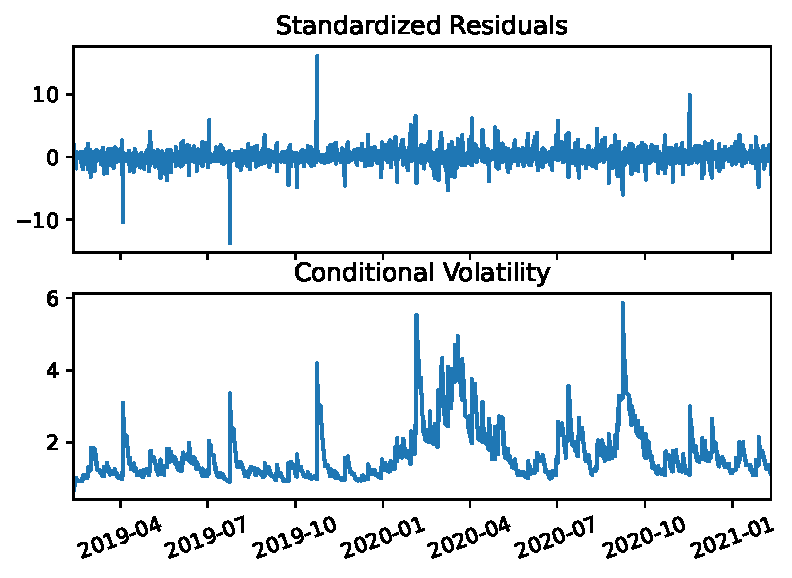
\includegraphics[width=\textwidth]{img/img_resid_garch.pdf}
	\caption{Standardized residual of the \acrshort{garch} fitting process and conditional volatility}
	\label{fig:resid_garch}
\end{figure}

\begin{figure}
	\centering
	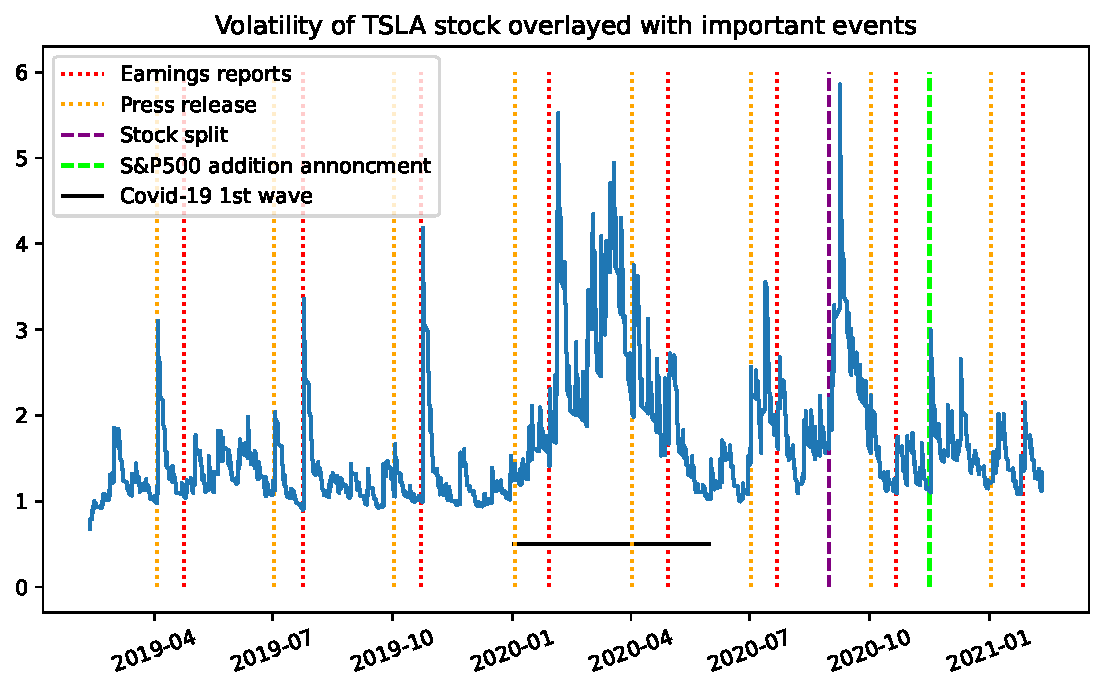
\includegraphics[width=\textwidth]{img/img_volatility_explanation.pdf}
	\caption{Important events overlayed with the \acrshort{garch} volatility}
	\label{fig:volatility_garch}
\end{figure}


The final \acrshort{ts} model is a \acrshort{garch}(1,1) model with Student-t distributed residuals. The parameters estimated by Python are:
\begin{align*}
\alpha_0 &= 0.042 \\
\alpha_1 &= 0.065 \\
\beta_1 &= 0.934 \\
\nu &= 2.56
\end{align*}
The parameters estimated by R are:
\begin{align*}
\alpha_0 &= 0.067 \\
\alpha_1 &= 0.137 \\
\beta_1 &= 0.935 \\
\nu &= 2.23 \\
\end{align*}

So there are some slight differences between the R and Python implementations, but the results are close. This could be explained by a difference of initial values for the solver


\section{Machine Learning Approach}

\chapter{Conclusion}

The \acrlong{ts} analysis shows that a \acrshort{garch}(1,1) model is good at explaining the stock price and it's fluctuations, and give us insight as to why and when the price fluctuates. Other than extreme events, such as the Covid-19 pandemic than created a sharp rise in volatility, there are some events, that occur at given times, know in advance, that create spikes in volatility. For example the quarterly earning reports. These spikes in fluctuation are important, as this is where people make or lose money in large quantities. Being able to consistently predict them, is an asset.

The \acrlong{ml} modeling and prediction shows that for default parameters, simple \acrlong{lm} still work the best. However I would like to have tuned the other methods, as this would greatly increase their accuracy and potentially yield better results than the \acrlong{lm}. I tried some manual tuning by varying the parameters of methods arbitrarily  and received some better results , but didn't spend enough time checking the tuning and being formal about it to include it in this report, out of fear that some results might just be coincidences and might mislead the reader.

We also see from the \acrlong{ml} approach, that the prediction get bad relatively fast after about one day in the future. 
My theory about this, other than the obvious that the more in the future we try to go, the more uncertainty there is, is the following. The frenzy (measured by Google Search activity and twitter activity) that makes price swing expires a lot faster than one week. My guess is it expires roughly after one day, and in our case, something probably happened 2 days or more after date from which we start predicting, and thus the relevant covariate information was not part of the input. This would explain why non of the models were able to predict the final spike in price.

As far as the comparison of Python and R, we were only able to do this with the \acrlong{ts} approach, and in this case the results very quite similar, with only minor differences. Explained probably by different choices in initial values or optimizers only, and not due to difference in implementation of methods in general. I was unable in the allocated time to get the R verison of the \acrlong{ml} to work, and so we can not do any comparison for those. I do suspect however that the results would be similar to those of Python as well.

As for a personal stand point, I came into this project with only a  little theoretical knowledge about the subject of \acrlong{ml} and one of my goals was to get a practical sense of how it worked and what needed to be done to get them to work. And this was fulfilled. I was surprised how much preprocessing of the data is necessary and how important it is. I also have a better understanding of the methods presented in the report even if not complete yet.

\chapter{Future Works}
To further this research, I would like to first and foremost tune the models and see what results I get with an optimal or close to optimal tuning.
Considering the dates of quarterly earnings report seem to have a big influence on the volatility of the process, as shown by the \acrlong{garch} fit, it might be worth taking that into account as a variable. I would also like to find other variables that could be good indicators of volatility more in advance than the Google searches, or tweet reactions.
Additionally, I would like to try more novel methods on this problem and see how well they would perform. Long Short-Term Memory models appear to show promise for modeling and predicting financial \acrlong{ts}, as seen in \cite{LSTMpaper1} or \cite{LSTMpaper2}
And finally , there is the possibility to shorten the prediction interval, as the methods work better on shorter time frames.

\chapter*{Code}
All code for this project can be found on \url{https://github.com/Sekarski/MasterThesis}

\begin{thebibliography}{9}

\bibitem{ARMAbook}
G. Box, G. Jenkins, \textit{Time Series Analysis: Forecasting and Control}, San Francisco, Holden-Day, 1970

\bibitem{ARCHpaper}
R. F. Engle, \textit{Autoregressive Conditional Heteroscedasticity with Estimates of the Variance of United Kingdom Inflation}, Econometrica, 50 (4), 987-1007, 1982

\bibitem{GARCHpaper}
T. Bollerslev, \textit{Generalized Autoregressive Conditional Heteroskedasticity} Journal of Economics, 31 (3), 307-327, 1986

\bibitem{DTpaper}
L. Breiman, J. H. Friedman, R. A. Olshen, C. J. Stone, \textit{Classification and regression trees}, Monterey CA: Wadsworth \& Brooks/Cole Advanced Books \& Software, 1984

\bibitem{RFpaper}
L. Breiman, \textit{Random Forests}, Machine Learning, 45(1),5-32, 2001

\bibitem{ETpaper}
P. Geurts, D. Ernst., and L.Wehenkel, \textit{Extremely randomized trees}, Machine Learning, 63(1),3-42,2006

\bibitem{LSTMpaper1}
Mehtab, Sen. \textit{Stock Price Prediction Using Machine Learning and LSTM-Based Deep Learning Models}, 2020

\bibitem{LSTMpaper2}
Ding, Qin. \textit{Study on the Prediction of Stock Price Based on the Associated Network Model of LSTM} International journal of machine learning and cybernetics 11.6 (2020): 1307–1317

\end{thebibliography}


\printglossary[type=\acronymtype]
\printglossary

\end{document}